%!TEX root = ../template.tex
%%%%%%%%%%%%%%%%%%%%%%%%%%%%%%%%%%%%%%%%%%%%%%%%%%%%%%%%%%%%%%%%%%%
%% chapter2.tex
%% NOVA thesis document file
%%
%% Chapter with introduction
%%%%%%%%%%%%%%%%%%%%%%%%%%%%%%%%%%%%%%%%%%%%%%%%%%%%%%%%%%%%%%%%%%%

\typeout{NT FILE chapter2.tex}%


\chapter{Atomic Structure Calculations}\label{cha:atom_calc}

In this chapter, the procedure that follows a standard atomic structure calculation will be discussed and explained in detail. Topics ranging from the usage of the \gls{MCDFGME} code to compute  quantities such as energy levels, orbital wavefunctions and transition rates, to the manner in which these parameters can be used in order to simulate a theoretical spectrum will be explored. All the information present in this chapter was obtained after a thorough study of \gls{MCDFGME}'s manual~\cite{Desclaux_Indelicato_2019}.


\section{The \gls{MCDFGME} code's capabilities}
As previously stated, \gls{MCDFGME} is a program that allows for not only solving the many-body problem for an atomic system while making the proper \gls{QED} energy corrections, but also for the computation of a great deal of atomic parameters. Consulting~\cite{mcdfWebsite}, one can see that these include, but are not limited to:

\begin{itemize}
    \item Energy level calculations.
    \item Multipole radiative transition probabilities.
    \item Auger transition probabilities.
    \item Photoionization cross-sections.
    \item Electronic impact excitation cross-sections.
    \item Orbital wavefunction overlaps between same and different atomic systems.
\end{itemize}
\todo{meter mais cenas}

% Quoting from the manual~\cite{Desclaux_Indelicato_2019}, these include:
% 
% \begin{itemize}
    % \item Total energy of a given state
    % \item Radiative and Auger transition probabilities
    % \item Photoionization cross-sections
    % \item Hyperfine structure constants
    % \item Landé factor
    % \item Electron impact excitation cross-sections
    % \item Stark effect
    % \item Parity non-conserving amplitude,
    % \item Magnetic part of the g 2 correction for antiprotons,
    % \item Scalar product of wave functions,
    % \item Shiff moment
    % \item Overlaps of orbitals between a n-electron and a n 1-electron state for Shake-off calculations
% \end{itemize}
%  


\section{The atomic system at study}

Before proceeding with the explanation behind every step of the calculations performed, a previous discussion on the objective of the following calculations should be had.


The main purpose of this thesis is that of simulating a theoretical spectrum for Copper's emission lines when subjected to a near ionization threshold x-ray source.

At this energy range, two main processes will be responsible for an electron moving out a core-shell: Resonant photoexcitation, and ionization.

While the simulation of the theoretical spectra for ionized Copper would be quite straightforward (due to the low shake probabilities at near ionization threshold energies, transitions for satellite states were not considered), the more extensive calculation is that of the resonant photoexcitation.

In order to fulfill the aim of simulating the theoretical spectra for this last phenomenon, multiple atomic structure calculations were computed for many of the excited state configurations for Copper.

In total, and in addition to ionized Copper, 18 different standalone calculations were performed for should the atomic system have gone through the process of an excitation of any one of the constituent electrons to the following orbitals:

\begin{itemize}
    \item 4s, 4p, 4d, 4f
    \item 5s, 5p, 5d, 5f, 5g
    \item 6s, 6p, 6d, 6f, 6g, 6h
    \item 7p, 8p, 9p
\end{itemize}


\subsection{Selecting all possible orbital configurations}
When performing an atomic structure calculation using the \gls{MCDFGME} code, a configuration needs to be given. Therefore, there is a need to manually
In order to perform an atomic structure calculation, by making use of the \gls{MCDFGME} code, the system's configuration is needed. This way, for each case, all the possible one-hole and two-holes configurations need to be provided, along with their respective labels which are used as identifiers of the orbital where the hole is present during the following calculations. For example, in the case of ground state Copper that went through the process of the excitation of one of its electrons to the orbital 4p, there are many possibilities for the original orbital from where the electron came from. For this case, an example of all possible 1-hole and 2-holes configurations can be found in Annex~\ref{ann:confs}. These are obtained by running a single, or two holes by all the orbitals present in the ground state configuration.


\section{Level Calculations}
Now that all configurations have been selected, the calculations can proceed.

The first step needed to be performed in order to simulate theoretical spectra is the calculation of the level structure for all given configurations.

This, however, is no simple task. Besides the given configuration, an atomic level is described by two other quantum numbers.

\subsection{The level manifold}




Prior to proceeding with the discussion, it is important to establish some of the notation that will be used throughout this thesis. In this work, an atomic level will be described by three sets of quantum numbers. These will be the parameters that will influence the system's energy level diagram.

\paragraph{Hole orbital labels}


$\qty(n\ l_j)$ - This set can be composed of one or more labels indicators of the subshell where holes are present.
For demonstrative purposes, assuming neutral Copper's ground state configuration as a starting point, before any hole-generating processes, to be $1\text{s}^2\ 2\text{s}^2\ 2\text{p}^6\ 3\text{s}^2\ 3\text{p}^6\ 3\text{d}^{10}\ 4\text{s}^1$, certain configurations can be obtained through the proper usage of the aforementioned quantum number set:

\begin{itemize}
    \item $1\text{s}^1\ 2\text{s}^2\ 2\text{p}^6\ 3\text{s}^2\ 3\text{p}^6\ 3\text{d}^{10}\ 4\text{s}^1  \rightarrow \qty(1\text{s})$
    \item $1\text{s}^1\ 2\text{s}^1\ 2\text{p}^6\ 3\text{s}^2\ 3\text{p}^6\ 3\text{d}^{10}\ 4\text{s}^1 \rightarrow \qty(1\text{s},2\text{s})$
\end{itemize}




\paragraph{Total angular momentum number}


$J$ - This number is the indicator of the total angular momentum of the atomic system, resulting from the couplings between the electrons'  orbital angular momenta and the electrons' spin. A single configuration can result in many coupling schemes, resulting in different couplings and, in turn, different values for $J$.

As an example, let's take that of Copper that went through the excitation process of an electron originally in the orbital 2p that is now in 4p, with an electron configuration of $1\text{s}^2\ 2\text{s}^2\ 2\text{p}^5\ 3\text{s}^2\ 3\text{p}^6\ 3\text{d}^{10}\ 4\text{s}^1\  4\text{p}^1 $. One can now easily observe there are three different open orbitals, each with an uncoupled electron. The different coupling possibilities between these three electrons will generate four different possible total angular momentum values: $J=\sfrac{1}{2},\ \sfrac{3}{2},\ \sfrac{5}{2},\ \sfrac{7}{2}$. In table \ref{tab:tot_ang_mom}, a coupling example will be given for each of them.


\begin{table}[h!]
    \centering
    \caption{Total angular momentum generated by different couplings}
    \label{tab:tot_ang_mom}
    \rowcolors{1}{}{GhostWhite}
    \begin{tabular}{cc| cc | cc|c}
        \toprule \multicolumn{2}{c|}{2p}&\multicolumn{2}{c|}{4s}&\multicolumn{2}{c|}{4p}&Total/$J$\\
        $m_l$ & $m_s$ & $m_l$&$m_s$&$m_l$&$m_s$&$m_l+m_s$\\\midrule
        $1$&$-\sfrac{1}{2}$&$0$&$-\sfrac{1}{2}$&$1$&$-\sfrac{1}{2}$&$\sfrac{1}{2}$\\
        $1$&$\sfrac{1}{2}$&$0$&$-\sfrac{1}{2}$&$1$&$-\sfrac{1}{2}$&$\sfrac{3}{2}$\\
        $1$&$\sfrac{1}{2}$&$0$&$\sfrac{1}{2}$&$1$&$-\sfrac{1}{2}$&$\sfrac{5}{2}$\\
        $1$&$\sfrac{1}{2}$&$0$&$\sfrac{1}{2}$&$1$&$\sfrac{1}{2}$&$\sfrac{7}{2}$\\
    \end{tabular}
\end{table}

\paragraph{Lagrange multiplier} $\epsilon$ - Indicator of the eigenvalue for the state on which the calculation will be performed on. The need for this quantum number arises from the fact that, even for the same configuration and the same total angular momentum, there are many possible arrangements that yield these quantum numbers. As an example, for the same configuration used previously, and assuming a total angular momentum $J=\sfrac{5}{2}$, there are three different possible couplings that generate that value of angular momentum, as can be seen in table \ref{tab:epsilon}.


\begin{table}[h!]
    \centering
    \caption{Same total angular momentum generated by different configurations}\label{tab:epsilon}
    \rowcolors{1}{}{GhostWhite}
    \begin{tabular}{cc| cc | cc}
        \toprule\multicolumn{6}{c}{$J=\sfrac{5}{2}$}\\\midrule
        \multicolumn{2}{c|}{2p}&\multicolumn{2}{c|}{4s}&\multicolumn{2}{c}{4p}\\
        $m_l$ & $m_s$ & $m_l$&$m_s$&$m_l$&$m_s$\\\midrule
        $1$&$-\sfrac{1}{2}$&$0$&$\sfrac{1}{2}$&$1$&$\sfrac{1}{2}$\\
        $1$&$\sfrac{1}{2}$&$0$&$-\sfrac{1}{2}$&$1$&$\sfrac{1}{2}$\\
        $1$&$\sfrac{1}{2}$&$0$&$\sfrac{1}{2}$&$1$&$-\sfrac{1}{2}$\\\bottomrule
    \end{tabular}
\end{table}

This splitting of quantum numbers for a given configuration gives origin to the level manifold (Figure~\ref{fig:manifold}), reason why, even for a simple calculation, hundreds to thousands of levels need to be calculated. It is also of note that, for a give Total angular momentum value, $J$, there are $2\times J+1$ states associated to it due to the angular momentum projection. In the presence of an external \gls{EMF}, the hyperfine level structure would be observed, due to Zeeman and Stark's effects. However, for the purpose of this thesis, no external field was considered, and a $2J+1$ degeneracy was taken into account in the following calculations.

\begin{figure}[h!]
    \centering
    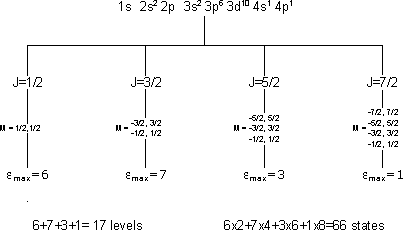
\includegraphics[width=\linewidth]{Chapters/Figures/Chapter2/1s_0_alt.pdf}
    \caption{Splitting of quantum numbers for a given configuration.}
    \label{fig:manifold}
\end{figure}

\begin{figure}[h!]
    \centering
    \begin{tikzpicture}
        \draw (0,0)node[anchor=south]{$1\text{s}^2\ 2\text{s}^2 2\text{p}^5\ 3\text{s}^2\ 3\text{p}^6\ 4\text{s}^1\ 4\text{p}^1\ $}--(0,-1);
        \draw (-6,-1) -- (6,-1);
        \draw (-6,-1) -- (-6,-2) node [anchor=north]{$J=\sfrac{1}{2}$};
        \draw (-2,-1) -- (-2,-2)node [anchor=north]{$J=\sfrac{3}{2}$};
        \draw (2,-1) -- (2,-2)node [anchor=north]{$J=\sfrac{5}{2}$};
        \draw (6,-1) -- (6,-2)node [anchor=north]{$J=\sfrac{7}{2}$};
        \draw (6,-2.5) -- (6,-3)node [anchor=north, text centered, align=center, text width=2cm]{
            $\sfrac{-7}{2},\ \sfrac{7}{2}$
            
            $\sfrac{-5}{2},\ \sfrac{5}{2}$

            $\sfrac{-3}{2},\ \sfrac{3}{2}$

            $\sfrac{-1}{2},\ \sfrac{1}{2}$
            };
        \node at (4.75,-4){$m_J =$};
        \draw (2,-2.5) -- (2,-3.25)node [anchor=north, text centered, align=center, text width=2cm]{
            $\sfrac{-5}{2},\ \sfrac{5}{2}$
            
            $\sfrac{-3}{2},\ \sfrac{3}{2}$

            $\sfrac{-1}{2},\ \sfrac{1}{2}$
            };
        \node at (0.75,-4){$m_J =$};
        \draw (-2,-2.5) -- (-2,-3.5)node [anchor=north, text centered, align=center, text width=2cm]{
            $\sfrac{-3}{2},\ \sfrac{3}{2}$
            
            $\sfrac{-1}{2},\ \sfrac{1}{2}$
            };
        \node at (-3.25,-4){$m_J =$};
        \draw (-6,-2.5) -- (-6,-3.75)node [anchor=north, text centered, align=center, text width=2cm]{
            $\sfrac{-1}{2},\ \sfrac{1}{2}$
            };
        \node at (-7.25,-4){$m_J =$};
        \node[white] at (7.25,-4){$m_J =$};

        \node at (-6,-6) {$6+7+3+1= 17$ levels};
        \node at (4,-6) {$6\times 2+7\times 4+3\times6+1\times 8=66$ states};
    \end{tikzpicture}
\end{figure}


associatedas
s
s
s
s
s
s
s


s
s

s

\todo{Breit can be used as self consistent or perturbative}


\subsubsection{Computing energy levels with \gls{MCDFGME}}



\section{Transition computations}
\subsection{Diagram transitions}
\subsection{Auger transitions}
\subsection{Satellite transitions}

\subsubsection{Rate Matrices as a calculation quality comparison tool}

